\section{Braitenberg Vehicles}

    Valentino Braitenberg (1926-2011) was an Italian neuroscientist and a synthetic psychologist. He spent most of his life doing experiments to understand how the animal nervous system works. He was also interested in building synthetic models of human or animal behaviour. He is well known for his book~\cite{braitenberg1986vehicles}. This book consists of a series of thought experiments about behaviours which can be expected of simple devices. All these thought experiments were inspired by animals and their nervous systems. He said ``when we analyse a mechanism, we tend to over-estimate its complexity".

    \subsection{Working of a Basic Braitenberg Vehicle}
    These are simple vehicles consisting of actively driven wheels and sensors. The sensors are stimulated by some stimulus (light, temperature, sound, presence of certain chemicals etc). The rotation speed of the wheels is directly controlled by the two sensor data. Depending upon how many sensors and wheels are there and how the sensor data influences the wheel speed (either excitatory or inhibitor), Braitenberg vehicles have been divided into the following categories:



    % Vehicle S1
    \subsubsection{Vehicle 1}
    \label{sec:Vehicle_1}

        \begin{figure}[t]%
            \centering
            \subfloat[\centering Excitatory Signal]{{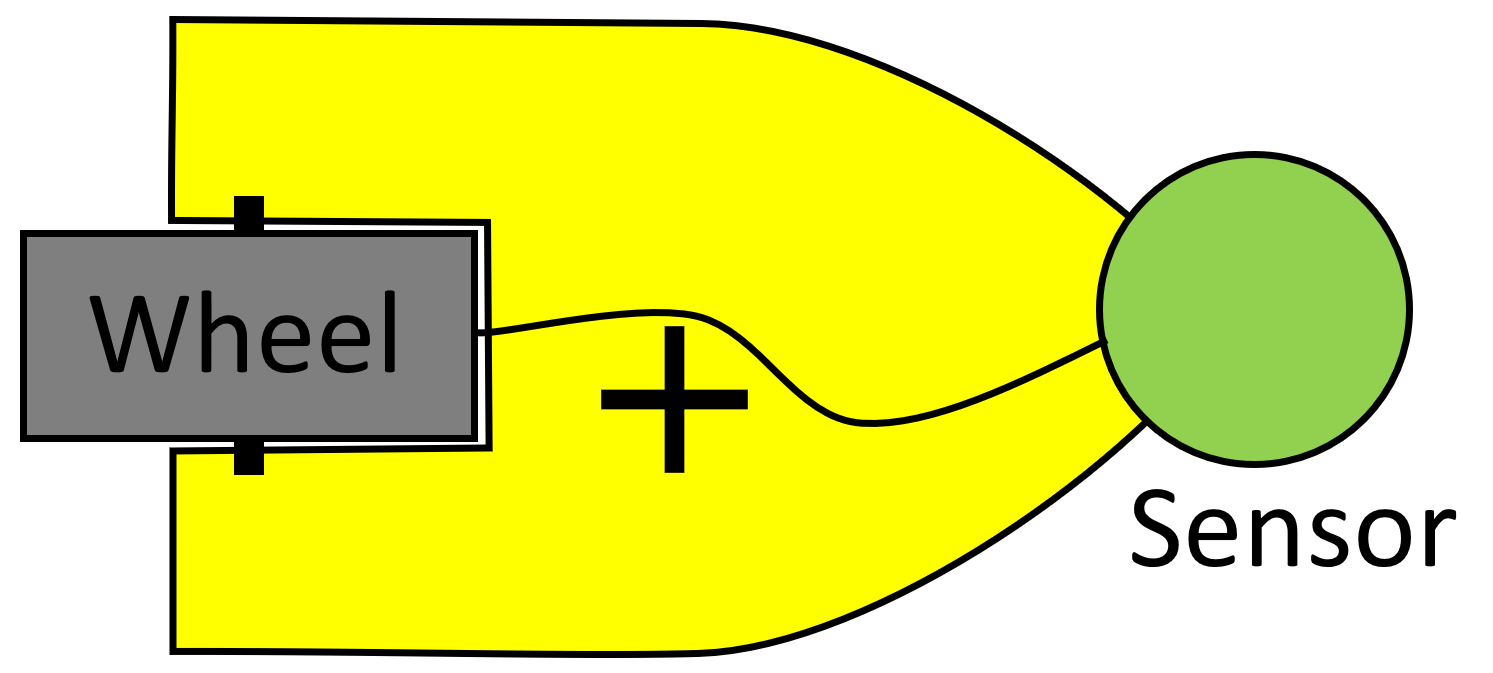
\includegraphics[width=5cm]{./images/1s_vehicle_p.png} }}%
            \qquad
            \subfloat[\centering Inhibitory Signal]{{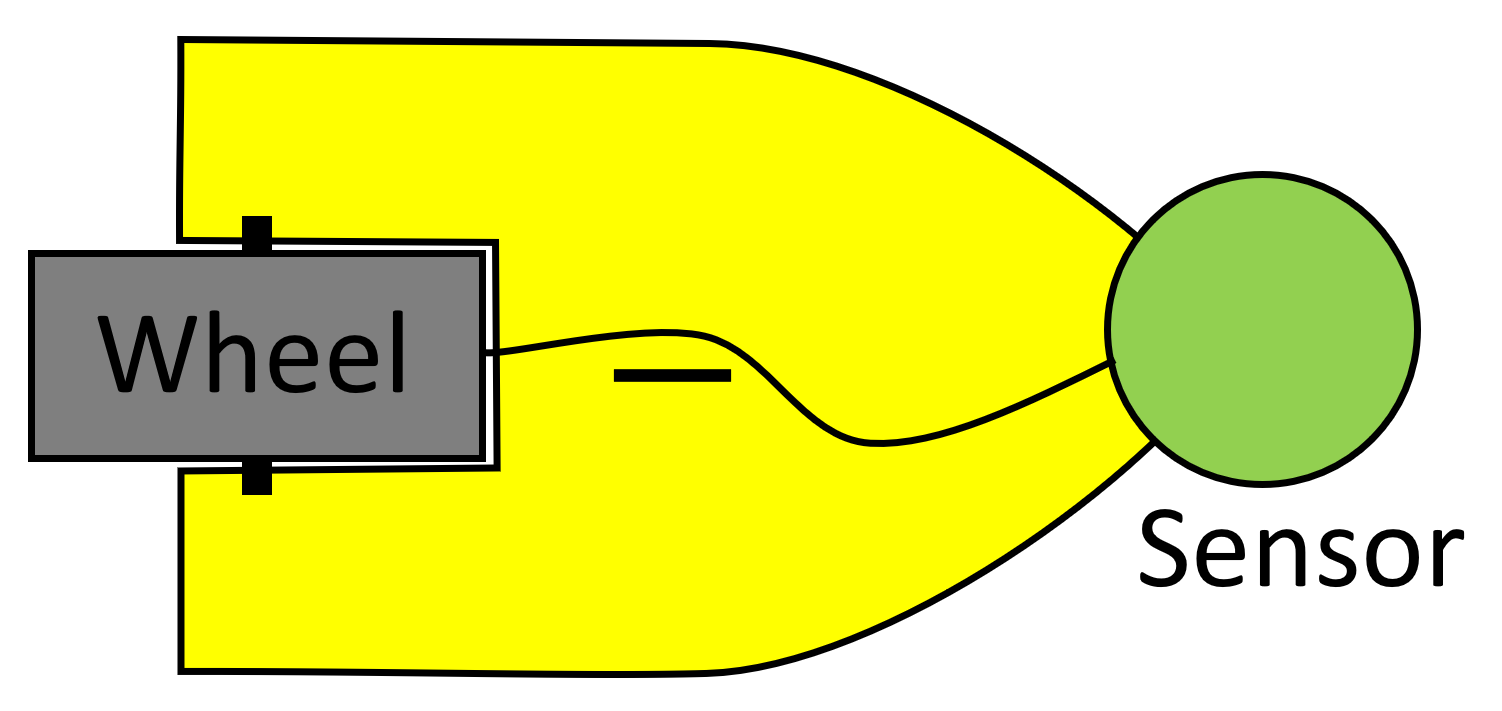
\includegraphics[width=5cm]{./images/1s_vehicle_m.png} }}%
            \caption{Braitenberg Vehicle Model 1}%
            \label{fig:vehicle1}%
        \end{figure}

        These vehicles (in Fig \ref{fig:vehicle1}) consist of a single sensor and a single wheel. These devices cannot change their directions. They move in a straight line. Now the sensor can either give an excitatory or an inhibitory signal to the wheel:

        \begin{itemize}
            \item \textbf{Excitatory Signal from Sensor:} Here, wheel speed is directly proportional to the strength of the stimulus. As the sensor senses more stimulus, (the stimulus is near) the wheel rotates faster; the vehicle gains speed. Thus, the speed of the vehicle is more when the vehicle is near the stimulus and the vehicle moves slowly when it is away from the stimulus. As a result, it spends less time near the source of stimulus and more time roaming away from it.
            \item \textbf{Inhibitory Signal from Sensor:} Here, wheel speed is inversely proportional to the strength of the stimulus. As the sensor senses more stimulus, the vehicle slows down. Thus, the devices gather around the source of stimulus.
        \end{itemize}


    % Vehicle S2
    \subsubsection{Vehicle 2}
    \label{sec:Vehicle_2}

        \begin{figure}[t]%
            \centering
            \subfloat[\centering Uncrossed Connection]{{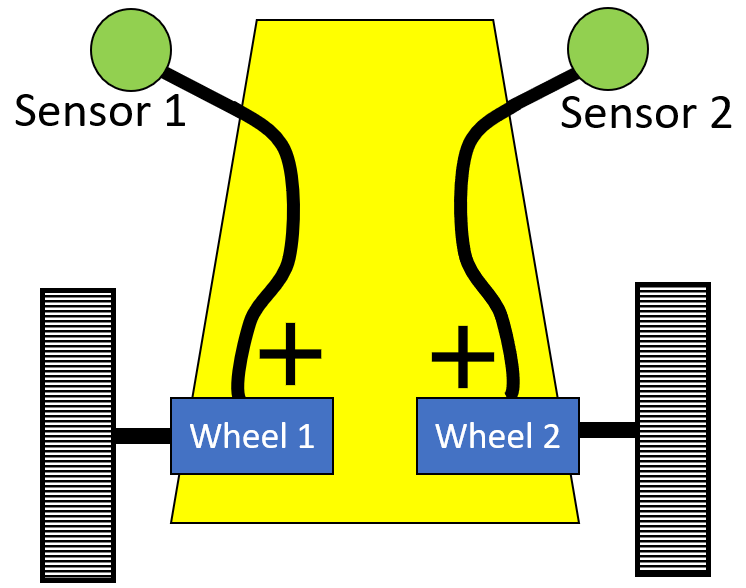
\includegraphics[width=5cm]{./images/2s_vehicle_d.png}}}%
            \qquad
            \subfloat[\centering Crossed Connection]{{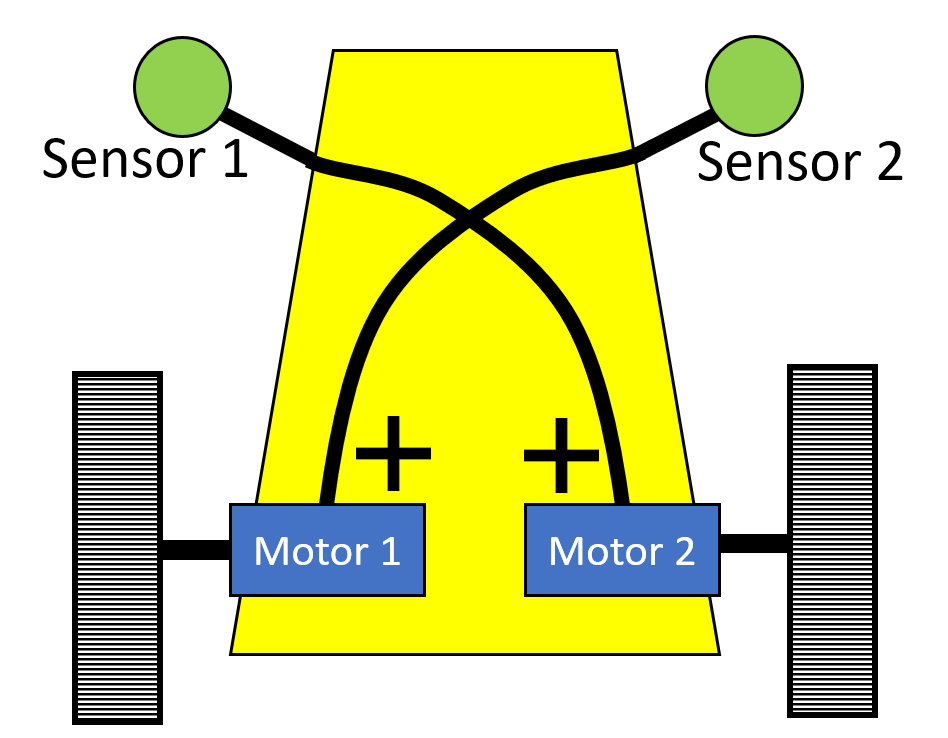
\includegraphics[width=5cm]{./images/2s_vehicle_c.png}}}%
            \caption{Braitenberg Vehicle Model 2}%
            \label{fig:vehicle2}%
        \end{figure}

        These vehicles (in Fig \ref{fig:vehicle2}) consist of two sensors and two wheels. Unlike \hyperref[sec:Vehicle_1]{Vehicle 1}, they can move freely on a 2D plane. But here, the sensors can always give an excitatory signal to the wheels. They have been divided into three categories depending upon their connections:

        \begin{itemize}
            \item \textbf{Uncrossed connections (2a):} Here, the left sensor is attached to the left wheel and the right sensor is attached to the right wheel. Now, suppose a source of stimulus is present on the right side of the vehicle, the right sensor is stimulated more than the left one. Hence the right wheel rotates faster than the left wheel. Thus the vehicle turns left and goes away from the stimulus.\\
            \textbf{Inference:} The vehicle expresses \textbf{fear} from the cause of the stimulus. And is termed as \textbf{`COWARD'} by Braitenberg.
            \item \textbf{Crossed connections (2b):} In this case, the left sensor is attached to the right wheel and the right sensor is attached to the left wheel. Now, to a stimulus on the right, the system responds by rotating the left wheel faster. It moves towards the stimulus. As it moves closer to the stimulus, its speed increases. Soon, the vehicle collides with the stimulus at great speed.\\
            \textbf{Inference:} The vehicle expresses \textbf{aggression/hate} towards the cause of the stimulus.
            \item \textbf{Double connections (2c):} Here, both the sensors are connected to both the wheels. As both the wheels symultaneously recieve the same signal, this vehicle cannot turn (turning is achieved by different speed of the wheels). Thus, despite having a more complex connection, the vehicle is inferior to both 2a and 2b vehicles.\\
            \textbf{Inference:} More complex connections do not always give us more complex functionality.
        \end{itemize}

        In general, all the types of Vehicle 2 dislike the presence of the stimulus in their vicinity.

    % Vehicle S3
    \subsubsection{Vehicle 3}
    \label{sec:Vehicle_3}

    \begin{figure}[t]%
        \centering
        \subfloat[\centering Uncrossed Connection]{{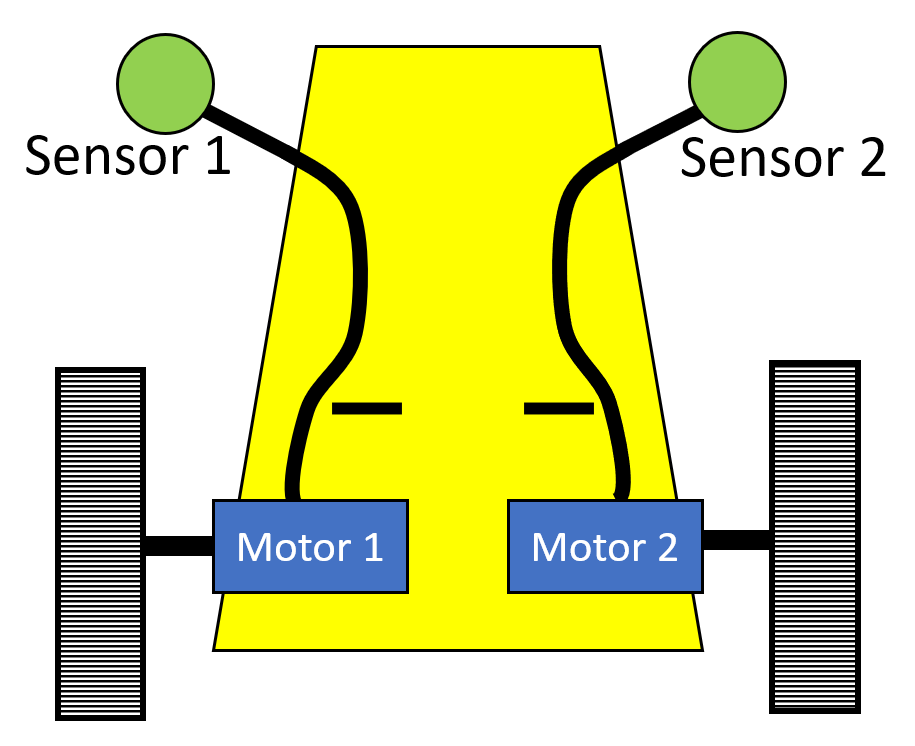
\includegraphics[width=5cm]{./images/3s_vehicle_d.png}}}%
        \qquad
        \subfloat[\centering Crossed Connection]{{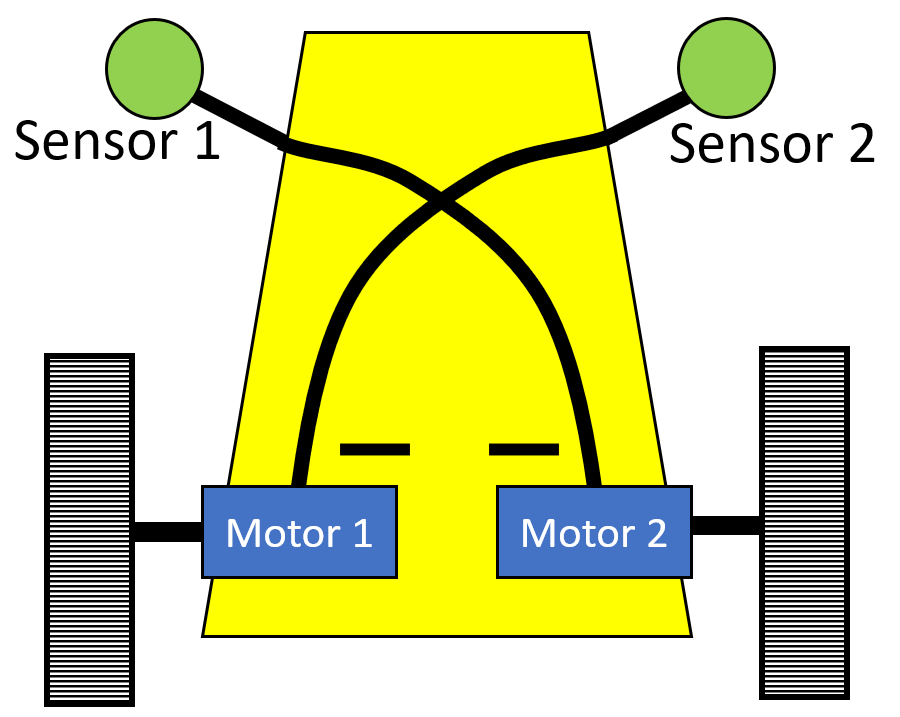
\includegraphics[width=5cm]{./images/3s_vehicle_c.png}}}%
        \caption{Braitenberg Vehicle Model 3}%
        \label{fig:vehicle3}%
    \end{figure}

    Just like the \hyperref[sec:Vehicle_2]{Vehicle 2} These vehicles (in Fig \ref{fig:vehicle3}) also have two sensors and two wheels. As a result, they also have full manoeuvring control over the plane (2D). But here, the sensors can always give an inhibitory signal to the wheels. In absence of a stimulus, the wheels rotate at full speed, and the speed decreases on detection of stimulus. Depending upon their connections, they are of 3 types:

    \begin{itemize}
        \item \textbf{Uncrossed connections (3a):} The sensors are connected to their respective wheels. A stimulus on the right side of the vehicle slows down the right wheel. Thus the vehicle turns right and turns toward the stimulus. After turning, it has the stimulus just in front of it. Hence, both the wheels slow down and move at the same speeds. The vehicle heads towards the stimulus. The strength of the stimulus increases. Speed of the vehicle decreases. Finally, it comes to a halt near the stimulus.\\
        \textbf{Inference:} The vehicle expresses \textbf{love} for the cause of the stimulus. It sticks to the first stimulus it sees in its life. It does not care about anything else, nor does it go to other, more powerful stimuli.
        \item \textbf{Crossed connections (3b):} The left wheel is slowed by the right sensor and the left sensor slows down the right wheel. In the presence of a stimulus, although it moves away from it, it slows down. It spends some time near the stimulus but eventually moves away in search of new, stimuli.\\
        \textbf{Inference:} Braitenberg describes this vehicle as an \textbf{explorer}.
    \end{itemize}

    Braitenberg talked about a lot of other sorts of vehicles. Some had different types of sensors attached to the same vehicle (maybe one pair of sensors detects temperature, another detects heat etc.) all of them give either positive or negative responses and may be connected in a crossed or uncrossed fashion. Some vehicles might have a different graph of influence (All this while we were talking about a proportional influence of sensors on wheels. But this might not always be the case. For example, an influence might be drastic, there is no slowing down - if the sensor receives a particular amount of stimulus, it completely turns the wheel on or off.). There are a lot of other types of simple vehicles discussed in detail by Braitenberg in his book. But this much discussion is enough for the purpose of this report.
